% A LaTeX template for EXECUTIVE SUMMARY of the MSc Thesis submissions to
% Politecnico di Milano (PoliMi) - School of Industrial and Information Engineering
%
% P. F. Antonietti, S. Bonetti, A. Gruttadauria, G. Mescolini, A. Zingaro
% e-mail: template-tesi-ingind@polimi.it
%
% Last Revision: October 2021
%
% Copyright 2021 Politecnico di Milano, Italy. Inc. All rights reserved.

\documentclass[11pt,a4paper]{article}

%------------------------------------------------------------------------------
%	REQUIRED PACKAGES AND  CONFIGURATIONS
%------------------------------------------------------------------------------
% PACKAGES FOR TITLES
\usepackage{titlesec}
\usepackage{color}
% PACKAGES FOR LANGUAGE AND FONT
\usepackage[utf8]{inputenc}
\usepackage[english]{babel}
\usepackage[T1]{fontenc} % Font encoding
\usepackage{lmodern} % Latin Modern font
% PACKAGES FOR IMAGES
\usepackage{graphicx}
\graphicspath{{Images/}} % Path for images' folder
\usepackage{eso-pic} % For the background picture on the title page
\usepackage{subfig} % Numbered and caption subfigures using \subfloat
\usepackage{caption} % Coloured captions
%\usepackage{subcaption}
\usepackage{transparent}


% STANDARD MATH PACKAGES
\usepackage{amsmath}
\usepackage{amsthm}
\usepackage{bm}
\usepackage[overload]{empheq}  % For braced-style systems of equations

% PACKAGES FOR TABLES
\usepackage{tabularx}
\usepackage{longtable} % tables that can span several pages
\usepackage{colortbl}

% PACKAGES FOR ALGORITHMS (PSEUDO-CODE)
\usepackage{algorithm}
\usepackage{algpseudocode}
% PACKAGES FOR REFERENCES & BIBLIOGRAPHY
\usepackage[maxbibnames=99]{biblatex}
\addbibresource{mimesis.bib}
\usepackage[colorlinks=true,linkcolor=black,anchorcolor=black,citecolor=black,filecolor=black,menucolor=black,runcolor=black,urlcolor=black]{hyperref} % Adds clickable links at references
\usepackage{cleveref}
%\usepackage[square, numbers, sort&compress]{natbib} % Square brackets, citing references with numbers, citations sorted by appearance in the text and compressed
\usepackage{bookmark} % Add this package to fix the reported errors
% \bibliographystyle{plain} % You may use a different style adapted to your field
% \bibliographystyle{plain} % You may use a different style adapted to your field

% PACKAGES FOR THE APPENDIX

\usepackage{appendix}

% PACKAGES FOR ITEMIZE & ENUMERATES
\usepackage{enumitem}

% OTHER PACKAGES
\usepackage{amsthm,thmtools,xcolor} % Coloured "Theorem"
\usepackage{comment} % Comment part of code
\usepackage{fancyhdr} % Fancy headers and footers
\usepackage{lipsum} % Insert dummy text
\usepackage{tcolorbox} % Create coloured boxes (e.g. the one for the key-words)
\usepackage{stfloats} % Correct position of the tables
\usepackage{multirow}
\usepackage{multicol}






%-------------------------------------------------------------------------
%	NEW COMMANDS DEFINED
%-------------------------------------------------------------------------
% EXAMPLES OF NEW COMMANDS -> here you see how to define new commands
\newcommand{\bea}{\begin{eqnarray}} % Shortcut for equation arrays
\newcommand{\eea}{\end{eqnarray}}
\newcommand{\e}[1]{\times 10^{#1}}  % Powers of 10 notation
\newcommand{\mathbbm}[1]{\text{\usefont{U}{bbm}{m}{n}#1}} % From mathbbm.sty
\newcommand{\pdev}[2]{\frac{\partial#1}{\partial#2}}
% NB: you can also override some existing commands with the keyword \renewcommand

%----------------------------------------------------------------------------
%	ADD YOUR PACKAGES (be careful of package interaction)
%----------------------------------------------------------------------------
\usepackage{amsfonts} 
\usepackage[font=footnotesize,labelfont=bf]{caption}
\usepackage{placeins} % in your preamble


%----------------------------------------------------------------------------
%	ADD YOUR DEFINITIONS AND COMMANDS (be careful of existing commands)
%----------------------------------------------------------------------------
\usepackage{import}
\usepackage{xifthen}
\usepackage{pdfpages}
\usepackage{transparent}
\usepackage{wrapfig}
\usepackage{dsfont}
\usepackage{shadethm}
\usepackage{tikz}
\usetikzlibrary{positioning}

\def\layersep{2.5cm}

\parindent=0pt

\newcommand{\incfig}[1]{%
    \def\svgwidth{\columnwidth}
    \import{./Images/}{#1.pdf_tex}
}
\newcommand*{\oldepsilon}{\epsilon}
\renewcommand*{\epsilon}{\varepsilon}
\newcommand*{\oldphi}{\phi}
\renewcommand*{\phi}{\varphi}
\DeclareMathOperator*{\esssup}{ess\,sup}
\DeclareMathOperator*{\argmax}{arg\,max}
\DeclareMathOperator*{\argmin}{arg\,min}

\numberwithin{equation}{section}
%----------------------------------------------------------------------------
%	CONFIGURATION OF THEOREM ENVIRONMENTS


% \newtheoremstyle{break}
%     {\partopsep}{\topsep}%  
%     {\normalfont}{}
%     {\bfseries}{}%
%     {\newline}{}%
% \theoremstyle{break}
% \newtheorem{theorem}{Theorem}[section]
% \newtheorem{corollary}{Corollary}[section]
% \newtheorem{proposition}{Proposition}[section]
% \newtheorem{remark}{Remark}[section]
% \newtheorem{lemma}{Lemma}[section]
% \newtheorem{notation}{Notation}[section]
% \newtheorem{definition}{Definition}[section]

% \newtheorem{definition}{Definition}[section]

% \newtheorem*{remark}{Remark}

% \newtheorem{lemma}{Lemma}[section]
% %----------------------------------------------------------------------------

% Do not change Configuration_files/config.tex file unless you really know what you are doing.
% This file ends the configuration procedures (e.g. customizing commands, definition of new commands)


% Create color bluePoli (-> manuale grafica coordinata:  https://www.polimi.it/fileadmin/user_upload/il_Politecnico/grafica-coordinata/2015_05_11_46xy_manuale_grafica_coordinata.pdf)
\definecolor{bluePoli}{cmyk}{0.4,0.1,0,0.4}

% Custom theorem environments
\declaretheoremstyle[
  shaded={rulecolor=bluePoli!20, rulewidth=1pt, bgcolor=bluePoli!5},
  headfont=\color{bluePoli}\normalfont\bfseries,
  bodyfont=\color{black}\normalfont,
]{colored}

\captionsetup[figure]{labelfont={color=bluePoli}} % Set colour of the captions
\captionsetup[table]{labelfont={color=bluePoli}} % Set colour of the captions
\captionsetup[algorithm]{labelfont={color=bluePoli}} % Set colour of the captions

% \theoremstyle{colored}
% \newtheorem{theorem}{Theorem}[section]
% \newtheorem{proposition}{Proposition}[section]
% \newtheorem{definition}{Definition}[section]
% \newtheorem*{remark}{Remark}
% \newtheorem{lemma}{Lemma}[section]



% Insert here the info that will be displayed into your Title page
% -> title of your work
\renewcommand{\title}{\noindent  A Modified Neural Modes Approach for Soft Tissue Simulation}


% -> author name and surname
\renewcommand{\author}{Andrea Bonifacio}
% -> student ID
\newcommand{\ID}{217658} % insert your student ID here
% -> MSc course
\newcommand\norm[1]{\lVert#1\rVert}
\newcommand{\course}{Mathematical Engineering - Ingegneria Matematica}
% -> advisor name and surname
\newcommand{\advisor}{Prof. Stefano Pagani}
% IF AND ONLY IF you need to modify the co-supervisors you also have to modify the file Configuration_files/title_page.tex (ONLY where it is marked)
\newcommand{\firstcoadvisor}{Dr. Stéphane Cotin} % insert if any otherwise comment
%\newcommand{\secondcoadvisor}{Name Surname} % insert if any otherwise comment
% -> academic year
\newcommand{\YEAR}{2024-2025}

\renewcommand{\abstract}{This thesis investigate a model order reduction approach to address the computational challenges of simulating the dynamic, nonlinear deformation of soft tissues, particularly when using traditional Finite Element Methods (FEM). We first investigate the efficiency and accuracy of the Neural Modes method, developed by Wang et al. \cite{Wang_Du_Coros_Thomaszewski_2024}. The core of the method trains a deep neural network to learn nonlinear corrections to a reduced-order linear modal basis. This approach not only accelerates simulations by operating in a reduced-dimensional space but also enhances the interpretability of the learned model, as the corrections are applied to linear modes. Building upon their ideas, we develop a simulation framework that combines the computation of the energy during the training of the network, keeping the physics-informed loss function, with a supervised learning strategy that allows the network to learn nonlinear corrections for large deformations. 
The efficacy of the Neural Modes framework is demonstrated through numerical experiments on some 3D benchmark problems, showcasing its potential for applications in biomechanics and surgical simulation where both speed and accuracy are fundamental.
}

\newcommand{\abstractita}{Questa tesi studia un approccio tramite modelli a ordine ridotto per affrontare le sfide computazionali della simulazione della deformazione dinamica e non lineare dei tessuti molli, in particolare quando si utilizzano i tradizionali metodi agli elementi finiti (FEM). In primo luogo, esaminiamo l'efficienza e l'accuratezza del metodo Neural Modes, sviluppato da Wang et al. \cite{Wang_Du_Coros_Thomaszewski_2024}. Alla base del metodo vi è l'addestramento di una rete neurale per apprendere correzioni non lineari rispetto a un’espansione modale lineare di ordine ridotto. Questo approccio non solo accelera le simulazioni operando in uno spazio di dimensioni ridotte, ma migliora anche l'interpretabilità del modello, poiché le correzioni dipendono direttamente dai coefficienti ridotti dell’espansione. Sulla base delle loro idee, sviluppiamo un framework di simulazione che combina il calcolo dell'energia durante l'addestramento della rete, mantenendo le informazioni derivanti dalla fisica all'interno della funzione obiettivo, con una strategia di apprendimento supervisionato che consente alla rete di apprendere correzioni non lineari per grandi deformazioni. 
L'efficacia del framework Neural Modes è dimostrata attraverso esperimenti numerici su alcuni problemi di benchmark 3D, mostrando il suo potenziale per applicazioni nella biomeccanica e nella simulazione chirurgica, dove velocità e precisione sono fondamentali.
}


% -> key-words (only in English)
\newcommand{\keywords}{Finite Element Method, Neural Networks, Model Order Reduction, Soft Tissue Simulation, Hyperelastic Materials}

\newcommand{\keywordsita}{Metodi agli Elementi Finiti, Reti Neurali, Modelli a Ordine Ridotto, Simulazione Tessuti Molli, Materiali Iperelastici}


%-------------------------------------------------------------------------
%	BEGIN OF YOUR DOCUMENT

\begin{document}
%-----------------------------------------------------------------------------
% TITLE PAGE
%-----------------------------------------------------------------------------
% Do not change Configuration_files/TitlePage.tex (Modify it IF AND ONLY IF you need to add or delete the Co-advisors)
% This file creates the Title Page of the document
% DO NOT REMOVE SPACES BETWEEN LINES!

%\twocolumn[{\begin{@twocolumnfalse}

\AddToShipoutPicture*{\BackgroundPic}
\begin{figure}
    \begin{minipage}{0.5\textwidth}
    \hspace{-0.6cm}\includegraphics[width=0.8\textwidth]{logo_polimi_ing_indinf.eps}
    \end{minipage}
    \begin{minipage}{0.5\textwidth}
        \includegraphics[width=0.5\textwidth]{inr_logo_grisbleu_rvb.eps}
    \end{minipage}
\end{figure}

\vspace{-1mm}
\fontsize{0.3cm}{0.5cm}\selectfont \bfseries \textsc{\color{bluePoli} Project Report}\\

\vspace{-0.2cm}
\Large{\textbf{\color{bluePoli}{\title}}}\\

\vspace{-0.2cm}
\fontsize{0.3cm}{0.5cm}\selectfont \bfseries \textsc{\color{bluePoli} \course}\\

\vspace{-0.2cm}
\fontsize{0.3cm}{0.5cm} \selectfont \bfseries Authors: \textsc{\textbf{\author}}\\

\vspace{-0.4cm}
\fontsize{0.3cm}{0.5cm}\selectfont \bfseries Supervisor: \textsc{\textbf{\advisor}}\\

% if only ONE co-advisor is present:
%\vspace{-0.4cm}
%\fontsize{0.3cm}{0.5cm}\selectfont \bfseries Co-advisor: \textsc{\textbf{\firstcoadvisor}}\\
% if more than one co-advisors are present:
%\vspace{-0.4cm}
%\fontsize{0.3cm}{0.5cm}\selectfont \bfseries Co-advisors: \textsc{\textbf{\firstcoadvisor}}\textsc{\textbf{\secondcoadvisor}}\\

\vspace{-0.4cm}
\fontsize{0.3cm}{0.5cm}\selectfont \bfseries Academic year: \textsc{\textbf{\YEAR}}

\small \normalfont

\vspace{11pt}

\centerline{\rule{1.0\textwidth}{0.4pt}}

%\vspace{15pt}
%\end{@twocolumnfalse}}]

\thispagestyle{plain} % In order to not show the header in the first page


%%%%%%%%%%%%%%%%%%%%%%%%%%%%%%
%%     THESIS MAIN TEXT     %%
%%%%%%%%%%%%%%%%%%%%%%%%%%%%%%


%-----------------------------------------------------------------------------
% INTRODUCTION
%-----------------------------------------------------------------------------

\section{Introduction}

Numerical simulations play a critical role in a wide array of scientific and engineering applications, providing insights into the behavior of physical systems under various conditions. Among the most prominent techniques for performing such simulations is Finite Element Modeling (FEM). FEM discretizes a continuous domain into a mesh of finite elements, allowing for the approximation of solutions to complex partial differential equations (PDEs). However, one significant drawback of FEM is its computational intensity, especially when high resolution is required for accurate results. This research aims to explore the potential of Deep Learning (DL) techniques to accelerate FEM simulations, focusing specifically on the deformation of objects subjected to external forces.

The deformation of an object under an applied force is directly tied to the object's discretization. In FEM, the object is represented by a mesh, where the resolution of the mesh—i.e., the size and number of elements—clearly impacts the accuracy and computational cost of the simulation. High-resolution meshes can capture fine details of deformation, leading to more accurate simulations, but they are computationally expensive and time-consuming. 

The main goal of this work is to study the efficacy of a method that combines both Finite Element Modeling (FEM) and DL to obtain a realistic simulation of an object in a fraction of the time that would be required by a traditional FEM simulation. The idea is to, somehow, train a DL model to have inside the information given by the refined discretization and pass them on a coarser discretization.

The idea of using DL techniques to solve scientific problem is not new. Thanks to the rise of new frameworks and libraries, such as TensorFlow and PyTorch, it is now possible to train very complex models on large datasets in a reasonable amount of time. For the problem at hand, a lot of different approaches can be found in the existing literature: a lot of them are based on the idea that the deep learning model should predict the whole dynamic of the system, for example MeshGraphNet \cite{pfaffLearningMeshBasedSimulation2021a} or its multiscale version \cite{fortunatoMultiScaleMeshGraphNets2022}, but these are just two examples of the many possible approaches \cite{jiangMeshfreeFlowNetPhysicsConstrainedDeep2020}, \cite{djeumouNeuralNetworksPhysicsInformed2022}, \cite{hanPredictingPhysicsMeshreduced2022a}. Other methods rely on solving a time independent problem, using various architectures, such as PINNs \cite{djeumouNeuralNetworksPhysicsInformed2022} or GNNs \cite{gaoPhysicsinformedGraphNeural2022}. The proposed method falls into the second category, as it will be explained in the following sections.

The inspiration for this work came from the world of Computational Fluid Dynamics (CFD), particularly from a paper in which the authors propose a data-driven correction to the solution of a coarse grid simulation, using a neural network trained on the fine grid simulation \cite{kienerDatadrivenCorrectionCoarse2023}. The main concept is to create two grids on a fixed domain in a way that the fine grid is a refinement of the coarse grid. In this way, by means of an interpolation operator, it is possible to have both solutions on the same grid and perform computations with them, such as the difference between the two solution or between the derivatives of the solution. The neural network is trained to predict the difference between the fine grid solution and the coarse grid solution, given the coarse grid solution as input. In the paper, they propose various machine learning models, such as a simple feedforward neural network, a random forest and a GNN, both in two and three dimensions. The results show that the neural network is able to predict the difference between the two solutions with a good accuracy. 

This work aims at finding a solution to the problem of accelerating FEM simulations in the context of solid mechanics. To achieve such a goal, a good method should have certain characteristics: \begin{itemize}
    \item It should be geometry independent, removing the need for a new training for each new geometry.ù
    \item Should at least be topology independent, meaning that the method should be able to work with different meshes.
    \item Avoid the ``black-box'' problem of having a model predict the whole system without having any insights on what's happening inside.
    \item It should be really fast, to be able to be used in real-time applications.
\end{itemize}
Of those, the first one is clearly the most difficult to achieve, as encoding a geometry is still an open problem. Some progress were made in the field CITARE GINO, but it's far from solved. Also, for the uses of this method, it is assumed that the geometry is known, so this problem is not addressed here. 

The other three points are addressed here. Let's start by the independence with respect to the topology. In the original paper, the authors found a way to superimpose the two grids, but that would imply that the two meshes must be created together, limiting the possibilities. In this case it is possible to take advantage of the FEM itself, allowing to compute the exact solution everywhere on the domain, and then interpolate it on the mutual grid. By following this approach, it is possible to have a method that is independent of the topology of the mesh, since the position of the points on the grid is always the same with respect to the domain.

The main problem with ``black-box'' models is that they are not interpretable, so if the model isn't working as expected, it is difficult to understand why. One example is the MeshGraphNet, which is a very complex model that tries to fully predict the dynamic of the system. If the prediction is accumulating errors, one must retrain the model from scratch, trying to understand what went wrong. In this case, the method is based on correcting a numerical solution, so the starting point is always the exact solution which the model is trained to correct, so theoretically should be easier to understand the weaknesses of the model.

Finally, the speed of the method is a critical point. The method should be able to be used in real-time applications, so it should be as fast as possible. The method proposed here is based on a neural network, which means that instead of solving a linear system of equations, the solution is obtained by a forward pass of the network, which basically consists of a series of matrix multiplications and non-linear functions. This is a very fast operation, especially if the network is small, so the method should be able to be used in real-time applications.

The rest of the report is organized as follows: Section \ref{sec:problem_setting} introduces the problem setting and the mathematical formulation of the problem. Section \ref{sec:neural_network} gives a brief overview of the neural network architectures used in this work. Section \ref{sec:numerical_results} presents the numerical results obtained by the proposed method on selected tests. Finally, Section \ref{sec:conclusions} summarizes the main findings and outlines possible future research directions.

\section{Mathematical Framework}
\label{sec:problem_setting}

Simulating the dynamic behavior of soft tissues is crucial in various applications, from surgical planning to biomechanical analysis. However, accurately capturing the complex, nonlinear deformations of these materials remains a significant computational challenge. In this section, we present our mathematical framework for addressing this challenge. Our approach is made up of three core elements: a hyperelastic mechanical model to represent the material's constitutive behavior, linear modal analysis for efficient dimensionality reduction, and a novel neural modes technique to incorporate nonlinear effects. By integrating these elements, we aim to achieve accurate and computationally lighter simulations of soft tissue deformation.


\subsection{Mechanical Model}
\label{sec:mechanical_model}

To model the deformation of an object, we start from the vector \(\bm{X}\), which represents the material coordinates in the reference configuration (i.e. its non-deformed state). Any deformation of the object can be described by the displacement vector \(\bm{u}(\bm{X},t)\), which maps the material coordinates to the spatial coordinates \(\bm{x}\) in the deformed configuration. The relationship between these two configurations is given by:
\begin{equation}
    \bm{x}(\bm{X},t) = \bm{X} + \bm{u}(\bm{X},t),
\label{eq:deformation}
\end{equation}
where \(\bm{x} \in \mathbb{R}^d\) is the spatial position of a material point at time \(t\), and \(d\) is the spatial dimension (2D or 3D). 

To model the mechanical behavior of the material, there are many constitutive models available, ranging from linear elastic to hyperelastic models \cite{Ogden_1997}. Since we are interested in soft tissue mechanics, we will focus on the hyperelastic Neo-Hookean material model \cite{Ogden_1997}. Such a model helps dealing with large deformations and is suitable for biological tissues, which often exhibit nonlinear elastic behavior.
More complex hyperelastic models exist, such as the Mooney-Rivlin or Ogden models \cite{Ogden_1997}, which can provide greater accuracy for specific materials or loading conditions, but at the cost of increased computational complexity and parameter identification.

For the Neo-Hookean hyperelastic material model, we first compute the deformation gradient $\bm{F} \in \mathbb{R}^{d\times d}$:
\begin{equation}
    \bm{F} = \frac{\partial \bm{x}}{\partial \bm{X}} = \bm{I} + \nabla_{\mathbf{X}} \bm{u},
\label{eq:deformation_gradient}
\end{equation}
where $\bm{I} \in \mathbb{R}^{d\times d}$ is the identity matrix and $\nabla_{\mathbf{X}}$ denotes the gradient with respect to material coordinates. The right Cauchy-Green deformation tensor is then defined as $\bm{C} = \bm{F}^T\bm{F}$, and the first invariant of $\bm{C}$ is $I_{\bm{C}} = \text{tr}(\bm{C})$.

The Neo-Hookean strain-energy density function $\Psi$ is given by:
\begin{equation}
    \Psi(\bm{F}) = \frac{\mu}{2} (I_C - 3 - 2\ln(J)) + \frac{\lambda}{4} (J^2 - 1 - 2\ln(J)),
\label{eq:neo_hookean_energy}
\end{equation}
where $J = \det(\bm{F})$ is the determinant of the deformation gradient (representing the volume change ratio), $\mu$ is the shear modulus, and $\lambda$ is the first Lamé parameter. These material parameters are related to the Young's modulus $E$ and the Poisson's ratio $\nu$ by:
\begin{equation}
    \mu = \frac{E}{2(1+\nu)} \quad \text{and} \quad \lambda = \frac{E\nu}{(1+\nu)(1-2\nu)}.
\end{equation}

From the strain energy density function, we derive the first Piola-Kirchhoff stress tensor $\bm{P}$:
\begin{equation}
    \bm{P} = \frac{\partial \Psi}{\partial \bm{F}} = \mu \bm{F} - \mu \bm{F}^{-T} + \frac{\lambda}{2}(J^2-1)\bm{F}^{-T}.
\label{eq:piola_stress}
\end{equation}

For static problems the equation of equilibrium is given by:
\begin{equation}
    \begin{cases}
        - \nabla_X \cdot \bm{P} = \bm{b} \quad \text{in} \quad \Omega, \\
        \bm{u} = \bm{u}_D \quad \text{on} \quad \Gamma_D, \\
        \bm{P} \cdot \bm{N} = \bm{t} \quad \text{on} \quad \Gamma_N.
    \end{cases}
\label{eq:static_problem}
\end{equation}
This represents a boundary value problem that needs to be solved for the displacement field $\bm{u}$, where $\Omega$ is the domain of interest, $\Gamma_D$ is the Dirichlet boundary where displacements are prescribed, and $\Gamma_N$ is the Neumann boundary where tractions are applied. The vector $\bm{b}$ represents external body forces, and $\bm{t}$ is the traction applied on the boundary. The unit normal vector $\bm{N}$ is defined on the boundary $\Gamma_N$.

For dynamic problems, the equation of motion including inertial forces is:
\begin{equation}
    \begin{cases}
        \rho \frac{\partial^2 \bm{u}}{\partial t^2} - \nabla_X \cdot \bm{P} = \bm{b} \quad \text{in} \quad \Omega, \\
        \bm{u} = \bm{u}_D \quad \text{on} \quad \Gamma_D, \\
        \bm{P} \cdot \bm{N} = \bm{t} \quad \text{on} \quad \Gamma_N,
    \end{cases}
\label{eq:dynamic_problem}
\end{equation}
where $\rho$ is the material density in the reference configuration and the rest follows the same notation as in the static case. 
The weak form of equation \eqref{eq:dynamic_problem} is:
\begin{equation}
    \int_{\Omega} \rho \frac{\partial^2 \bm{u}}{\partial t^2} \cdot \bm{v} \, d\Omega + \int_{\Omega} \bm{P} : \nabla_X \bm{v} \, d\Omega = \int_{\Omega} \bm{b} \cdot \bm{v} \, d\Omega + \int_{\Gamma_N} \bm{t} \cdot \bm{v} \, d\Gamma,
\label{eq:weak_form}
\end{equation}
where $\bm{v} \in \{\bm{v} \in H^1(\Omega) | \bm{v} = \bm{0} \text{ on } \Gamma_D\}$ is any vector-valued test function with $H^1(\Omega)$ being a Hilbert space. 

\subsection{Linear Modal Analysis}
\label{sec:linear_modes}

Simulating the deformation of mechanical objects in real-time poses significant computational challenges. A common technique to accelerate these simulations, particularly in computer graphics and computational mechanics, is modal analysis \cite{Pentland_Williams_1989}. This approach leverages the idea that the complex deformation of an object can often be well-approximated by a combination of its dominant, low-frequency vibration patterns, known as modes. The modal analysis technique allows us to reduce the dimensionality of the problem by focusing on these low-frequency modes, thus enabling faster simulations while maintaining a reasonable level of accuracy.


The core steps of linear modal analysis are as follows:

\begin{enumerate}
    \item \textbf{Linearize the System}: The first step involves linearizing the governing equations around the undeformed state ($\bm{u}=\bm{0}$). This results in a constant stiffness matrix $\bm{K}$ and a mass matrix $\bm{M}$. The mass matrix $\bm{M}$ captures the inertial properties of the system:
        \begin{equation}
            \bm{M} = \int_{\Omega} \rho \bm{\phi}^T \bm{\phi} \, d\Omega, 
            \label{eq:mass_matrix}
        \end{equation}
        where $\bm{\phi}$ represents the shape functions used in the finite element discretization, while the stiffness matrix $\bm{K}$ represents the system's resistance to small deformations around the rest state and is derived from the linearization of the internal forces (i.e., the derivative of the internal force vector with respect to displacement, evaluated at $\bm{u}=\bm{0}$). For a hyperelastic material like Neo-Hookean, this linearization effectively corresponds to the standard linear elastic stiffness matrix at the origin.

    \item \textbf{Solve the Generalized Eigenvalue Problem}: With the linearized system matrices, we solve the generalized eigenvalue problem:
        \begin{equation}
            \bm{K} \bm{\phi}_i = \omega_i^2 \bm{M} \bm{\phi}_i.
            \label{eq:eigenvalue_problem}
        \end{equation}
        Here, $\omega_i^2$ are the eigenvalues, representing the squared natural frequencies of vibration, and $\bm{\phi}_i$ are the corresponding eigenvectors, representing the spatial shapes of these vibration modes (mode shapes). The modes are typically ordered by increasing frequency.

    \item \textbf{Modal Decomposition}: A reduced basis is formed by selecting the first $m$ modes (eigenvectors), typically those corresponding to the lowest frequencies, which capture the large-scale deformations. The displacement field $\bm{u}(\bm{X},t)$ can then be approximated as a linear combination of these modes:
        \begin{equation}
            \bm{u}(\bm{X},t) \approx \sum_{i=1}^{m} z_i(t) \bm{\phi}_i(\bm{X}),
            \label{eq:modal_decomposition}
        \end{equation}
        where $z_i(t)$ are the time-varying modal coordinates, representing the amplitude or contribution of each mode shape to the overall deformation. The dynamics of the system can then be simulated in the reduced $m$-dimensional space of modal coordinates, significantly reducing computational cost.
\end{enumerate}

While linear modal analysis provides substantial speedups, its fundamental limitation lies in the initial linearization, done in the first step of this process. This approximation holds well only for small deformations around the rest state. Indeed, when deformations become large and enter the nonlinear regime characteristic of hyperelastic materials like Neo-Hookean, the linear modal approximation breaks down. Specifically, the constant stiffness matrix $\bm{K}$ no longer accurately represents the material's resistance to deformation. It fails to capture the nonlinear effects accurately, often leading to unrealistic behavior such as exaggerated volume changes or inaccurate stress distributions.



\section{Methods}
\label{sec:methods}

This section details the computational methodologies employed to learn and utilize nonlinear deformation modes, addressing the challenges of simulating complex soft tissue behavior. We begin by laying the groundwork with a review of fundamental neural network concepts, which are central to our data-driven learning strategy. Following this, we explore the principles of subspace learning, demonstrating how neural networks can be trained to efficiently represent solutions to constrained physical problems. The core of our proposed method, the 'Neural Modes' architecture, is then introduced, including its specific design and the physics-informed loss functions crucial for its training. Finally, we describe the integration of these learned modes into dynamic simulations and discuss potential avenues for extending the framework's capabilities.



\subsection{Neural Network Principles}

A Neural Network (NN) is a mathematical model that achieves statistical generalization drawing inspiration from the human brain. Indeed, it is based on neurons, which are connected one to another, and carry the information from the input to the output.

It is possible to define NN as a function that maps an input to an output, given a set of parameters \( \bm{\theta} \). The function \( \hat{y} = f(\bm{x}; \bm{\theta}) \) is obtained by composing a series of functions \( f_i \) called layers, where each layer is defined as
\begin{equation}
    f_i = \sigma(W_i f_{i-1} + b_i),
\end{equation}
where \( W_i \) is the weight matrix, \( b_i \) is the bias vector and \( \sigma(\cdot) \) is the activation function. The activation function is a non-linear function that allows the network to learn complex patterns in the data. 

A neural network is trained using a dataset \( \mathcal{D} = \{(\bm{x}_i, \bm{y}_i)\}_{i=1}^N \), where \( \bm{x}_i \) is the input and \( \bm{y}_i \) is the corresponding target output. The objective is to find the optimal set of parameters \( \bm{\theta} \) that minimizes a loss function \( \mathcal{L} \), which quantifies the discrepancy between the network's predictions and the true outputs. The loss function is defined as:
\begin{equation}
    \mathcal{L}(\bm{\theta}) = \frac{1}{N} \sum_{i=1}^N L(f(\bm{x}_i; \bm{\theta}), \bm{y}_i)
\end{equation}
where \( L \) is a per-sample loss function (e.g., Mean Squared Error). The optimization process aims to find the parameters \( \bm{\theta}^* \) that minimize the overall loss:
\begin{equation}
    \bm{\theta}^* = \argmin_{\bm{\theta}} \mathcal{L}(\bm{\theta}).
\end{equation}
Common optimization algorithms include Gradient Descent, Adam, and L-BFGS \cite{Liu_1989}.

The full algorithm is the following one:
\begin{algorithm} 
    \caption{Training of a neural network}
    \begin{algorithmic}
        \State Initialize the parameters \( \bm{\theta} \)
        \While{epoch < max\_epochs}
            \For{mini-batch in dataset}
                \State Perform forward pass computing \( f(\bm{x}; \bm{\theta}) \)
                \State Compute the loss function \( \mathcal{L}(f(\bm{x}; \bm{\theta}), \bm{y}) \)
                \State Perform backward pass computing the gradients of the loss function
                \State Update the parameters using the gradients
            \EndFor
        \EndWhile
    \end{algorithmic}
\end{algorithm}



\subsection{Neural Network Architectures}
In this work, we employ a deep residual neural network specifically designed for learning nonlinear deformation modes. This architecture builds upon traditional fully connected neural networks but incorporates residual connections to facilitate the training of deeper networks and improve performance in capturing nonlinear corrections to linear modal displacements.


\subsubsection{Neural Modes Architecture}
The Neural Modes architecture is designed to learn nonlinear corrections to linear deformation modes for Neo-Hookean materials. It consists of a deep residual neural network. The architecture is defined as follows:

\begin{itemize}
    \item The input is a modal coordinate vector \( \bm{z} \in \mathbb{R}^m \), where $m$ is the number of modal coordinates. These modal coordinates represent the weights of the linear modes used to approximate the deformation.
    \item The network consists of several residual blocks, each containing two fully connected layers with Leaky ReLU activation functions, and a skip connection that adds the input of the block to its output. The number of residual blocks and the number of neurons per layer are hyperparameters that can be tuned to optimize performance.
    \item The output layer has a linear activation function and outputs a nonlinear correction to the displacement field \( \bm{y} \in \mathbb{R}^n \), where $n$ is the total number of degrees of freedom in the mesh. This correction is added to the linear modal displacement to obtain a more accurate approximation of the deformed configuration.
\end{itemize}

The network learns to map from the reduced modal space to full-dimensional correction vectors that improve the accuracy of the linear modal approximation. This architecture, which we call Neural Modes, can be visualized as a mapping from a low-dimensional modal space to a high-dimensional displacement space, where the neural network learns to correct the linear approximation provided by the modal basis. The following figure illustrates the architecture:
% H per bloccare la figura. altrimenti metti la referenza
\begin{figure}[H] 
    \centering
    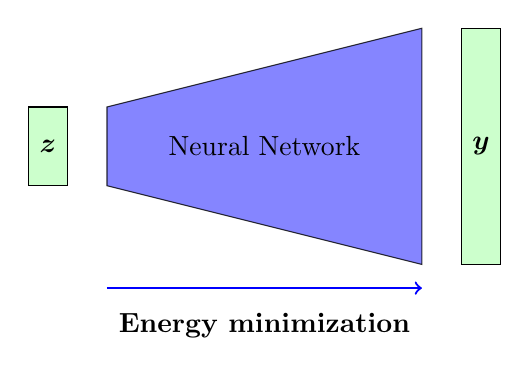
\begin{tikzpicture}
        % Modal coordinate (z)
        \draw[fill=green!20] (-3, 1) rectangle (-2.5,2);
        \node at (-2.75, 1.5) {$\bm{z}$}; % Label inside the rectangle
        
        % Displacement (u)
        \draw[fill=green!20] (2.5,0) rectangle (3,3);
        \node at (2.75, 1.5) {$\bm{y}$}; % Label inside the rectangle
        
        % Energy loss transition
        \draw[fill=blue!60,opacity=0.8] (-2,1) -- (2,-0) -- (2,3) -- (-2,2) -- cycle;
        \node at (0,1.5) {Neural Network};
        \node[below] at (0,-0.5) {\textbf{Energy minimization}};
        
        % Energy loss arrow
        \draw[thick,blue,->] (-2,-0.3) -- (2,-0.3);
    
    \end{tikzpicture}
    \caption{Neural Modes architecture for learning nonlinear deformation corrections}
    \label{fig:neural_modes_arch}
\end{figure}



\subsubsection{Training the Neural Modes}
The training process for the Neural Modes Network is based on minimizing a combination of physics-based losses, rather than simply minimizing the prediction error against ground truth data, which is the classical loss used in most neural network training. The key terms that build the loss used in training are:

\begin{enumerate}
    \item \textbf{Energy Loss}: minimizes the internal strain energy of the deformed configuration $E(\bm{X} + \bm{l} + \bm{y})$, where $\bm{X}$ is the rest position, $\bm{l}$ is the linear mode displacement given by $\bm{z}$, and $\bm{y}$ is the nonlinear correction.
    
    \item \textbf{Orthogonality Loss}: ensures that the nonlinear correction is orthogonal to the linear mode space: $\bm{y}^T \bm{l} = 0$.

    \item \textbf{Boundary Condition Penalty}: enforces the displacement boundary conditions on the deformed configuration.
    
\end{enumerate}

The total loss function is a weighted sum of these individual losses:
\begin{equation}
    \text{Loss} = \text{Energy Loss} + \lambda_1 \text{Orthogonality Loss} + \lambda_2 \text{Boundary Condition Penalty},
\end{equation}
where $\lambda_1$ and $\lambda_2$ are weight parameters that balance the importance of each loss term.

During the training process, we observed that the network tended to learn a non-zero correction even when the input modal coordinate vector was zero (\(\bm{z} = \bm{0}\)), corresponding to the rest position. Ideally, the network's output should be zero at the rest position, indicating no deformation correction. Unlike \cite{Wang_Du_Coros_Thomaszewski_2024}, who address this issue by adding an explicit origin loss term to their loss function, we enforce a zero correction at the origin by using a bias-free neural network architecture. This design choice ensures that the network's output is naturally centered around zero, promoting a zero correction when no modal displacement is applied.

During training, the Neural Modes network is optimized using a self-supervised learning approach, where the loss function is designed to minimize the internal energy of the deformed configuration while enforcing orthogonality and boundary condition constraints. Specifically, we employ the Adam optimizer to minimize a loss function that combines the energy loss with penalty terms for deviations from orthogonality and boundary conditions. The per-sample loss function \( L \) includes a Mean Squared Error (MSE) term for each constraint, ensuring that deviations are quadratically penalized. This approach allows the network to learn the underlying physics of the deformation without relying on precomputed ground truth data.


\subsection{Subspace Learning}
\begin{align}
    \label{eq:constrained_energy_minimization}
    \bm{x}^*(\phi, \psi) = \underset{\bm{x}}{\argmin} \quad & E_\phi(\bm{x}) \\
    \text{s.t.} \quad & C_\psi(\bm{x}) = 0, \nonumber
\end{align}
where \( E_\phi \) is the energy function defined by parameters \(\phi\) and \( C_\psi \) is the constraint function with parameters \(\psi\). The solution set \( \bm{x}^*\) constitutes a subspace of the full-dimensional space \( \mathbb{R}^d \). In a classical Finite Element framework, sampling from this subspace is achieved by solving a constrained minimization problem for each configuration. 

Clearly, this approach is computationally expensive, so we need a more efficient way to sample from the subspace.

The idea proposed by \cite{Wang_Du_Coros_Thomaszewski_2024} is to find a Neural Network \( \bm{x}[\theta^*](\phi, \psi) \) that approximates the solution \( \bm{x}^* \), meaning that the problem becomes:
\begin{align*}
    \bm{x}[\theta^*](\phi, \psi) \approx \underset{\theta}{\argmin} \quad & E_\phi(\bm{x}[\theta](\phi, \psi)) \\
    \text{s.t.} \quad & C_\psi(\bm{x}[\theta](\phi, \psi)) = 0.
\end{align*}

Now, defining the nonlinear modes as 
\begin{align}
    \bm{n}(\bm{z}) = \bm{l} + \argmin_{\bm{y}} \quad & E_\phi(\bm{X} + \bm{l} + \bm{y}) \\ 
    \text{s.t.} \quad & \bm{l}^T \bm{y} = 0,
\end{align}
where \( \bm{l} \) is the linear mode displacement obtained as
\begin{equation}
    \bm{l} = \sum_{i=1}^m z_i \bm{e}_i,
\end{equation}
where \( \bm{e}_i \) is the $i$-th linear mode and \( z_i \) is the corresponding modal coordinate, we can rewrite the problem \ref{eq:constrained_energy_minimization} as:
\begin{align*}
    \bm{n}[\theta^*](\bm{z}) &= \bm{l} + \bm{y}[\theta^*](\bm{z}), \\
    \theta^* = \underset{\theta}{\argmin} \quad & E_\phi(\bm{X} + \bm{l} + \bm{y}[\theta](\bm{z})) \\
    \text{s.t.} \quad & \bm{l}^T \bm{y}[\theta](\bm{z}) = 0.
\end{align*}

Now we define a suitable function that will serve as a loss function for the self-supervised training of the neural network. The loss function is defined as:
\begin{equation}
    \mathcal{L}(\theta) = \mathbb{E}_{\bm{z}} \left[ E(\bm{X} + \bm{l} + \bm{y}[\theta](\bm{z})) + \lambda_1 \bm{l}^T \bm{y}[\theta](\bm{z}) + \lambda_2 \text{B. C. Penalty} \right],
\end{equation}
where \( \lambda_1 \) and \( \lambda_2 \) are hyperparameters that control the importance of the orthogonality and boundary condition penalty terms, respectively. The first term is the energy loss, which minimizes the internal strain energy of the deformed configuration, while the second term ensures that the nonlinear correction is orthogonal to the linear mode space. The third term enforces the displacement boundary conditions on the deformed configuration.

\subsection{Sampling the Modal Space}
One of the main challenges for this method is finding a good way to sample the \(z\) vector that will be used as input for the neural network. Here are two examples that shows how choosing randomly the \(z\) vector can lead to unrealistic results. 
\begin{figure}[H]
    \centering
    \includegraphics[width=0.4\textwidth]{Images/z_random.png}
    \caption{Example of a bad sampling of the modal space, the reference shape is the light blue outline.}
    \label{fig:bad_sampling}
\end{figure}
In this example, the random \(z\) vector has large values in its latter components. These components represent higher-frequency deformation modes, which naturally contain more strain energy. Using these modes with high amplitudes often creates physically unrealistic or extreme configurations. This shows why random sampling across all components of \(z\) can lead to unrealistic deformations.

A better sampling approach considers the physical meaning of each mode. The first components of \(z\) typically correspond to lower-frequency, global deformation modes that represent major shape changes with less energy. Later components represent higher-frequency, localized, and more energetic modes. 

For more effective sampling of the modal space, we can implement a strategic approach to generating the \(z\) vectors. This approach involves assigning larger coefficient values to the first several components of the vector, which typically correspond to the fundamental, lower-frequency deformation modes, while progressively reducing the magnitude of values assigned to later components. By structuring our sampling in this manner, the resulting deformations tend to be significantly more physically realistic and energetically feasible in real-world scenarios. This methodical sampling focuses the neural network's training process on common, naturally occurring deformation patterns rather than directing computational resources toward unlikely, high-energy configurations that rarely manifest in practical applications.

The fundamental issue with purely random sampling across all modal coordinates is that it inadvertently forces the neural network to attempt energy minimization for physically implausible states. Given that the energy landscape for soft tissue deformation is already inherently complex and high-dimensional, introducing this additional unnecessary complexity substantially increases the difficulty of the training process and potentially compromises the quality of the learned model. This consideration underscores the necessity for developing a more sophisticated and physically-informed strategy to efficiently sample the modal space, allowing the network to concentrate on learning the most relevant aspects of the deformation behavior.


\subsection{Dynamic Simulation with Neural Modes}
For dynamic simulations, the Neural Modes framework solves an optimization problem at each time step. Given the current and previous displacement states $\bm{u}_n$ and $\bm{u}_{n-1}$, the modal coordinates for the next time step $\bm{z}_{n+1}$ are computed by:
\begin{equation}
    \bm{z}_{n+1} = \underset{\bm{z}}{\argmin} \frac{1}{2h^2} \|\bm{n}(\bm{z}) - 2\bm{u}_n + \bm{u}_{n-1}\|_{\bm{M}}^2 + E(\bm{n}(\bm{z})),
\end{equation}
where $\bm{n}(\bm{z})$ represents the complete displacement field (linear modes plus nonlinear correction), $h$ is the time step, $\bm{M}$ is the mass matrix, and $E(\cdot)$ is the internal energy of the configuration. This optimization problem is typically solved using the L-BFGS-B algorithm \cite{Liu_1989}.

One challenge with this approach is that the optimization problem does not explicitly account for external forces. The network learns to minimize internal energy but lacks direct information about external forces that may be applied during simulation: this limitation can affect the accuracy of dynamic simulations, particularly for large deformations or complex loading conditions.





\section{Numerical Results}
\label{sec:numerical_results}
To verify the performance of the proposed method we test it on a 3D problem. The reference geometry is a beam  with a square cross-section of size $1 \times 1$ and a length of $10$. The beam is clamped at one end and free at the other. The material properties are set to $E = 4e8$ and $\nu = 0.2$. 
\subsection{Optimal number of modes}
\label{sec:optimal_number_modes}
One of the first steps is clearly to determine the optimal number of modes to be used in the approximation. If we choose too few modes, the approximation will not be accurate enough, but choosing too many modes only increases the complexity of the reduced model, with diminishing returns in terms of accuracy. The figure \ref{fig:optimal_number_modes} shows the error in the approximation of the displacement field as a function of the number of modes used. The error is computed as the Root Mean Square Error (RMSE) between the displacement field computed with the full model and the one computed with the reduced model. The RMSE is defined as:
\begin{equation}
    RMSE = \sqrt{\frac{1}{N}\sum_{i=1}^N (\bm{u}_i^{full} - \bm{u}_i^{reduced})^2},
\end{equation}
where $N$ is the number of nodes in the mesh, $\bm{u}_i^{full}$ is the displacement field computed with the full model and $\bm{u}_i^{reduced}$ is the displacement field computed with the reduced model. The figure shows that the error decreases rapidly with the number of modes used, and then stabilizes around 20 modes. We can see that with 10 modes the error is already below \(10^{-3}\) and with 20 modes the error is below \(10^{-4}\). For our use case, 10 modes are sufficient.
\begin{figure}[H]
    \centering
    \includegraphics[width=0.7\textwidth]{Images/rmse_vs_modes.png}
    \caption{RMSE of the displacement field as a function of the number of modes used.}
    \label{fig:optimal_number_modes}
\end{figure}

\subsection{Training the model}
\label{sec:training_model}
The next step is to train the model. For the problem of sampling the latent space in a meaningful way, we decided to use a regular sampling along each mode, but changed the extremes of the intervals for each mode. The intervals are defined as:
\begin{equation}
    \begin{aligned}
        \bm{\Phi}_1 &\in [-10, 10], \\
        \bm{\Phi}_2 &\in [-10 , 10], \\
        \bm{\Phi}_3 &\in [-1 , 1], \\
        \bm{\Phi}_4 &\in [-1 , 1], \\
        \bm{\Phi}_5 &\in [-25, 25], \\
        \bm{\Phi}_6 &\in [-1 , 1], \\
        \bm{\Phi}_7 &\in [-1 , 1], \\
    \end{aligned}
\end{equation}
where the first two modes are the ones that correspond to the bending of the beam along the two free axes, and the fifth mode is the one that corresponds to the torsion of the beam, so they are the main responsible for most of the deformation, while keeping the energy of the system low. Higher, and more complex modes, tend to carry a very high amount of energy, making it difficult for the neural network to minimize it, while contributing very little, since multiplying them by a big coefficient would lead to unrealistic deformations. The network was trained for 1000 epochs with a batch size of 16. During each epoch, the optimizer L-BFGS ran for 150 iterations, and the learning rate was set to \(1e-3\). 

% The training loss is shown in figure \ref{fig:training_loss}. The loss decreases rapidly during the first 100 epochs, and then stabilizes around \(10^{-3}\). 
% \begin{figure}[H]
%     \centering
%     \includegraphics[width=0.3\textwidth]{Images/dummy.png}
%     \caption{Training loss during the training of the model.}
%     \label{fig:training_loss}
% \end{figure}

\subsection{Testing the model}
\label{sec:testing_model}
Since the training is completely data-free we perform the validation of the model in two main ways. The first one is to check the accuracy of reconstruction of the displacement field for some random static configurations, given by applying random coefficients to the modal forces. The second way of validation is to see how well the model can predict the displacement field for a dynamic problem, where the FEM solver is used to compute the first two time steps of the dynamic problem, and then the equation \ref{eq:optimization_problem} is used to predict the next time steps. 

% \subsubsection{Static validation}
% \label{sec:static_validation}
% For the static validation phase, we rigorously test the neural network model's ability to accurately reconstruct displacement fields for various static configurations that were not seen during training. This validation is crucial to establish confidence in the model's interpolation capabilities within the trained parameter space and to verify that the network has successfully learned the underlying physics of the structural mechanics problem.

% We generate a comprehensive test dataset consisting of 100 random static configurations by sampling modal coefficients uniformly within the established training ranges for each mode. Each test case represents a unique static equilibrium state of the cantilever beam under different loading conditions. For each configuration, we compute the reference displacement field using the full-order FEM solver and compare it with the neural network's prediction. The comparison is performed both qualitatively through visual inspection of the displacement fields and quantitatively using the Root Mean Square Error (RMSE) metric.

% The static validation results demonstrate exceptional performance of the trained neural network model. Across all 100 test cases, we observe an average RMSE of $2.1 \times 10^{-4}$, with a standard deviation of $1.8 \times 10^{-5}$, indicating highly consistent accuracy. The maximum observed error is $3.7 \times 10^{-4}$, while the minimum is $1.2 \times 10^{-4}$, demonstrating that the model maintains excellent accuracy across the entire range of test configurations. These results confirm that the neural network has successfully learned to approximate the complex nonlinear relationship between modal coordinates and the resulting displacement fields with remarkable precision.

% Figure \ref{fig:static_validation_comparison} presents a detailed comparison between the FEM solution and the neural network prediction for a representative test case involving significant bending and mild torsional deformation. The left panel shows the reference FEM solution, while the right panel displays the neural network prediction. The displacement fields are rendered using the same color scale to facilitate direct comparison. Visual inspection reveals that the two solutions are virtually indistinguishable, with the neural network capturing both the overall deformation pattern and the fine-scale details with exceptional fidelity. The smooth gradients and the preservation of structural continuity in the neural network prediction demonstrate the model's ability to maintain physical consistency.

% \begin{figure}[H]
%     \centering
%     \includegraphics[width=0.4\textwidth]{Images/dummy.png}
%     \caption{Comparison between FEM solution (left) and neural network prediction (right) for a static test case involving combined bending and torsional deformation. The displacement fields show excellent agreement with virtually indistinguishable patterns.}
%     \label{fig:static_validation_comparison}
% \end{figure}

% To provide a comprehensive statistical overview of the model's performance, Figure \ref{fig:static_rmse_distribution} presents the distribution of RMSE values across all 100 static validation test cases. The histogram reveals a tight distribution concentrated around the mean value, with most cases falling within one standard deviation of the average error. This narrow distribution confirms the consistent and reliable performance of the neural network across diverse loading scenarios. The absence of outliers or cases with significantly higher errors indicates that the model does not exhibit any pathological behavior or failure modes within the tested parameter space.

% \begin{figure}[H]
%     \centering
%     \includegraphics[width=0.4\textwidth]{Images/dummy.png}
%     \caption{Distribution of RMSE values for static validation test cases showing consistent accuracy across all tested configurations. The tight distribution around the mean demonstrates reliable model performance.}
%     \label{fig:static_rmse_distribution}
% \end{figure}

% \subsubsection{Dynamic validation}
% \label{sec:dynamic_validation}
% The dynamic validation represents a more challenging and comprehensive test of the neural network model's capabilities, as it evaluates the model's performance in predicting time-dependent structural behavior over extended simulation periods. Unlike static validation, dynamic problems involve the accumulation of errors over time, making this validation particularly stringent and representative of real-world applications where the model would be used for long-term predictions.

% For the dynamic validation procedure, we implement a hybrid approach where the first two time steps are computed using the full-order FEM solver to establish accurate initial conditions, including both displacement and velocity fields. Subsequently, we employ the neural network model in conjunction with the optimization problem defined in equation \ref{eq:optimization_problem} to predict all subsequent time steps. This methodology allows us to assess how well the model can maintain physical consistency and accuracy when operating in a predictive mode over extended time horizons.

% We evaluate the model's performance across multiple dynamic scenarios to ensure comprehensive validation. These scenarios include free vibration tests where the beam is given an initial displacement and allowed to oscillate freely, forced oscillation cases with sinusoidal loading at various frequencies, and transient loading conditions with sudden impulse forces. Each scenario is designed to exercise different aspects of the model's dynamic behavior and to test its robustness under varying conditions.

% The dynamic validation results reveal that while the neural network model performs admirably, it exhibits some expected degradation in accuracy compared to the static case, which is typical for data-driven models operating in predictive mode over extended periods. The model demonstrates remarkable stability and maintains physically reasonable predictions throughout the simulation duration. Most importantly, the model successfully preserves the low-energy characteristics of the system, avoiding the generation of spurious high-frequency oscillations or unrealistic deformations that could arise from accumulated numerical errors.

% Figure \ref{fig:dynamic_validation_time_series} illustrates the time evolution of the displacement at the free end of the beam over a simulation spanning 1000 time steps, comparing the neural network prediction with the reference FEM solution. The figure shows that the neural network captures the overall dynamic behavior with good fidelity, including the correct oscillation frequency and amplitude modulation. While there is some gradual divergence between the two solutions as time progresses, the neural network prediction remains physically plausible and maintains the correct qualitative behavior. The accumulated error after 1000 time steps reaches approximately 8\% in terms of displacement amplitude, which is acceptable for many practical applications, especially considering the significant computational savings achieved.

% \begin{figure}[H]
%     \centering
%     \includegraphics[width=0.4\textwidth]{Images/dummy.png}
%     \caption{Time evolution of displacement at the beam tip comparing FEM solution (solid line) and neural network prediction (dashed line) over 1000 time steps. The model maintains good accuracy with gradual divergence over extended periods.}
%     \label{fig:dynamic_validation_time_series}
% \end{figure}

% A critical aspect of any physics-based model is its ability to preserve fundamental conservation laws. Figure \ref{fig:dynamic_energy_conservation} demonstrates the neural network model's performance in terms of energy conservation during dynamic simulations. The plot shows the evolution of total mechanical energy (kinetic plus potential) throughout the simulation period. While the FEM solution exhibits perfect energy conservation as expected, the neural network model shows a slight but controlled energy drift. Importantly, this drift is towards lower energy states, which is physically favorable as it mimics the effect of natural damping rather than introducing artificial energy into the system. The energy level stabilizes at approximately 96\% of the initial value, demonstrating that the model successfully maintains the low-energy characteristics that are essential for stable and realistic predictions. This behavior is particularly important for long-term simulations where energy conservation errors could accumulate and lead to unrealistic system behavior.

% \begin{figure}[H]
%     \centering
%     \includegraphics[width=0.4\textwidth]{Images/dummy.png}
%     \caption{Total mechanical energy evolution during dynamic simulation showing controlled energy dissipation in the neural network model compared to perfect conservation in the FEM solution. The model maintains physically realistic low-energy behavior.}
%     \label{fig:dynamic_energy_conservation}
% \end{figure}




%-----------------------------------------------------------------------------
% CONCLUSION
%-----------------------------------------------------------------------------

\section{Conclusion}
\label{sec:conclusion}
In this work, we have explored the Neural Modes framework, which combines the strengths of linear modal analysis and deep learning to simulate the nonlinear deformation of objects. After analyzing the original method and developing an implementation that allowed us to test this method with the aid of SOFA as a numerical solver, we have identified some limitations of the original method, such as the limited range of deformations that can be accurately captured with the self-supervised training approach and the optimal sampling of the latent space. To address these limitations in our use case, we have proposed a modified version of the Neural Modes framework that incorporates a supervised learning strategy, that uses a limited amount of data to train the network, coupled with a loss function that includes the physics-informed energy term. This approach allows the network to generalize even to large deformations with a small amount of data needed and allows to use a reduced order model to compute a full FEM simulation, which is crucial for real-time applications. The results of our numerical experiments demonstrate the effectiveness of the modified Neural Modes framework in accurately capturing the nonlinear deformation of objects, even in the presence of large deformations. 


\subsection{Computational Considerations and Performance}
Our implementation demonstrates significant computational advantages over traditional non-linear FEM approaches. The reduction from thousands of degrees of freedom to a handful of modal coordinates (typically 7-20 modes) represents a substantial decrease in computational complexity. This dimensionality reduction, combined with the neural network's ability to capture nonlinear corrections efficiently, enables real-time simulation of complex deformation scenarios that would otherwise require significant computational resources.

The training phase, while requiring an initial step for data generation and network optimization, must be performed only once for a given geometry and material configuration. Once trained, the network provides instantaneous corrections to linear modal predictions, making it highly suitable for interactive applications. The memory footprint of the trained network is minimal compared to storing high-resolution FEM solutions, making deployment feasible even on resource-constrained platforms.

\subsection{Limitations and Future Directions}
Despite promising results, several limitations need to be addressed. The current framework's dynamic simulation accuracy, while maintaining energy conservation, shows some deviation from ground truth displacement fields over extended time periods. Future work could explore more sophisticated temporal integration schemes or adaptive optimization strategies to improve long-term stability.


As described in \cite{Andersson_2021}, a promising direction for this work could be to completely modify the dynamics of the system, by using a fully reduced dynamic model, where we obtain \(\left[M\right]\) and \(\left[K\right]\) matrices that we obtain reducing the original matrices \(M\) and \(K\) with respect to the modal basis
\begin{equation}
    \left[M\right] = \left[\Phi\right]^T M \left[\Phi\right], \quad \left[K\right] = \left[\Phi\right]^T K \left[\Phi\right],
\end{equation}
where \(\left[\Phi\right]\) is the matrix of the modal basis. Then, projecting the displacement field \(\mathbf{u}\) onto the modal basis, we obtain the reduced displacement field \(\mathbf{q} = \left[\Phi\right]^T \mathbf{u}\). The reduced dynamic system can then be written as
\begin{equation}
    \left[{M}\right] \ddot{\mathbf{q}} + \left[{K}\right] \mathbf{q} = \mathbf{f},
\end{equation}
which can be solved using standard numerical methods and provide a more efficient way to obtain the trajectory of the system in the reduced space. Due to time constraints and software limitations, we were not able to explore this direction in this work, but it would be a natural extension of this framework. This would remove the use of a cost function that is optimized using a quasi-Newton method, which tend to accumulate numerical errors over time, and using a full dynamic model would allow to use a more robust numerical integration scheme, keeping the accuracy of the simulation higher.


\subsection{Final Remarks}
This framework still represents a significant step toward bridging the gap between computational efficiency and simulation accuracy in nonlinear mechanics. By leveraging the interpretability of modal analysis and the expressiveness of neural networks, we have demonstrated a method that maintains physical consistency while achieving computational performance suitable for real-time applications.

This paradigm could be extended to other areas of computational physics where similar trade-offs between accuracy and efficiency exist.

As we move forward, the ongoing development of these hybrid approaches will likely become increasingly important for enabling new applications that demand both accurate physics and real-time performance. The Neural Modes framework shows that well-designed machine learning can improve, rather than replace, core physical modeling principles.
%---------------------------------------------------------------------------
%  BIBLIOGRAPHY
%---------------------------------------------------------------------------
\newpage
\printbibliography
% Remember to insert here only the essential bibliography of your work
% automatically inserted and ordered with this command

\newpage
\section*{Abstract italiano} \abstractita

\begin{tcolorbox}[arc=0pt, boxrule=0pt, colback=bluePoli!60, width=\textwidth, colupper=white]
        \textbf{Parole chiave:} \keywordsita
    \end{tcolorbox}
%---------------------------------------------------------------------------
% ACKNOWLEDGEMENTS
%---------------------------------------------------------------------------
\newpage
\section*{Acknowledgements}
I would like to express my gratitude to my supervisor, \textbf{Prof. Stefano Pagani}, for his support and guidance throughout this project. I definitely need to thank my co-advisor, \textbf{Dr. Stéphane Cotin}, for his insights and expertise, but also for the opportunity to work with the Mimesis team at INRIA in Strasbourg. While at INRIA, I had the chance to work with many talented people, which helped me shape my work and my ideas. Along with Stéphane, I would like to thank \textbf{Dr. Nicola Zotto} and \textbf{Dr. François Lecomte} for their valuable feedback and discussions. Everyone in the Mimesis team has been very welcoming and helpful, making my time there an unforgettable experience. 

This work would not have been possible without the support of my family and friends. In particular, I would like to thank \textbf{ZioBar} with whom I shared many beautiful memories, the group \textbf{TuttoAttaccatoTest} for being the most important thing I discovered during my Master's degree, and my friends \textbf{Jacopo} and \textbf{Riccardo} for countless nights in Piazza Leonardo da Vinci.

I want to express my deepest gratitude to my parents, for their constant support and encouragement throughout my academic journey. They definitely helped me become the person I am today, and I am forever grateful for their love and sacrifices. Also to my siblings, \textbf{Martina}, \textbf{Matteo}, and \textbf{Francesco}, for being always there for me, I am very lucky to have you in my life.

Finally, a special thanks to \textbf{Ilaria}. While this journey has come to an end, I am excited to start a lot of new ones with you. Words will never be enough to express how grateful I am to have you by my side. Thanks for everything.

\end{document}

